\chapter{Estado de la Cuestión}
\label{cap:estadoDeLaCuestion}

En este capítulo, se estudiarán detalladamente las simulaciones basadas en agentes de inteligencia artificial y modelos de lenguaje, así como las complejidades en las relaciones sociales y la interacción persona-ordenador. El objetivo fundamental es contextualizar la evolución histórica y actual de estos temas, destacando la relevancia de su estudio y desarrollo, subrayando la importancia de que estos sistemas puedan ser fácilmente extensibles y utilizados por profesionales de distintos ámbitos. El capítulo se dividirá en varios puntos, los cuales se pueden englobar en dos secciones.

La primera sección del estado de la cuestión se centra en las simulaciones basadas en agentes y su aplicación en entornos de inteligencia artificial. Se explorarán los avances tecnológicos, las metodologías y los desarrollos más recientes que han influido en la creación de sistemas de simulación avanzados. Asimismo, se examinará la relación de estos agentes con modelos de lenguaje, identificando los desafíos de esta convergencia tecnológica.

Después, se revisarán los desarrollos más destacados en procesamiento del lenguaje natural (PLN) y cómo estos contribuyen a la mejora de la interacción entre humanos y sistemas de inteligencia artificial. Además, se explorarán los aspectos psicológicos relacionados con las relaciones sociales en el contexto de la informática. También se centrará en la interacción persona-ordenador, se analizarán las tendencias actuales en diseño centrado en el usuario y las estrategias para garantizar que las simulaciones de inteligencia artificial sean accesibles a todos los públicos, independientemente de su desconocimiento sobre la tecnología.

\section{Simulaciones basadas en agentes}
\section{Modelos de lenguaje}
\subsection{Generativos}
\subsection{LLM}
\section{Agentes}

\section{Procesamiento del lenguaje natural}

El procesamiento del lenguaje natural (PLN) es una rama de la inteligencia artificial que se enfoca en la interacción entre las computadoras y el lenguaje humano. El objetivo del PLN es permitir que las máquinas comprendan y procesen el lenguaje humano de la misma manera que lo hacemos los seres humanos. Esto lo consiguen combinando la lingüística computacional con modelos estadísticos de machine learning y deep learning, pudiendo así interpretar tanto datos de texto como de voz, e incluso imágenes u otros tipos.

\subsection{Historia del PLN}

Se podría considerar el 1950 como el año de surgimiento del PLN, con la publicación de \cite{10.1093/mind/LIX.236.433}, donde se proponía el conocido \textit{Test de Turing}, una herramienta que evalúa la capacidad de una máquina para exhibir un comportamiento inteligente similar o indistinguible al de un ser humano, teniendo a una persona como evaluadora del comportamiento y comparando las respuestas con las de un humano real. Esto abrió el debate sobre si las máquinas eran o no capaces de "pensar" y sobre cómo pueden interpretar el texto que reciben y devolver una salida que cobre sentido.

Entre finales de los años 70 y el año 1985, surgieron modelos que se basaban en reglas para realizar traducciones automáticas, ya que en la época, era el principal objetivo del PLN, como Syntra \citep{Toma1970SYSTRANMT}. A principios del siglo XXI se vio que estos sistemas no eran los más eficientes y, a partir de los años 2010, s empezó a emplear el método de la inteligencia artificial para el procesamiento del lenguaje natural.

En la actualidad, las investigaciones en PLN se centran en mejorar la capacidad de las máquinas para comprender el contexto y la intención detrás del lenguaje humano. Avances notables incluyen el desarrollo de modelos de lenguaje preentrenados, como BERT (Bidirectional Encoder Representations from Transformers) y GPT (Generative Pre-trained Transformer), que han demostrado una capacidad excepcional para captar la complejidad del lenguaje natural \citep{devlin2019bert}.

A día de hoy, estos sistemas han sido perfeccionados y se utilizan de manera habitual en varios ámbitos como pueden ser la recuperación y extracción de información, la minería de datos, la traducción automática, el análisis de sentimientos o la generación de resúmenes automáticos \citep{hernandez2013aplicaciones}. En el caso de este estudio, es especialmente interesante la generación de resúmenes automáticos, ya que es una de las extensiones propuestas en los objetivos de realización del trabajo.

\subsection{PLN para resúmenes de textos}

En los últimos años, se han propuesto diversos generadores de secuencias. En particular, los que más éxito han tenido son los basados en arquitecturas de aprendizaje profundo (deep learning) \citep{mishra2020deep}. Las definiciones de la figura \ref{fig:resumenTextos} se refieren a los distintos tipos de resúmenes de textos que pueden existir, según \cite{adhikari2020nlp}. 

\begin{figure}[h]
	\centering
	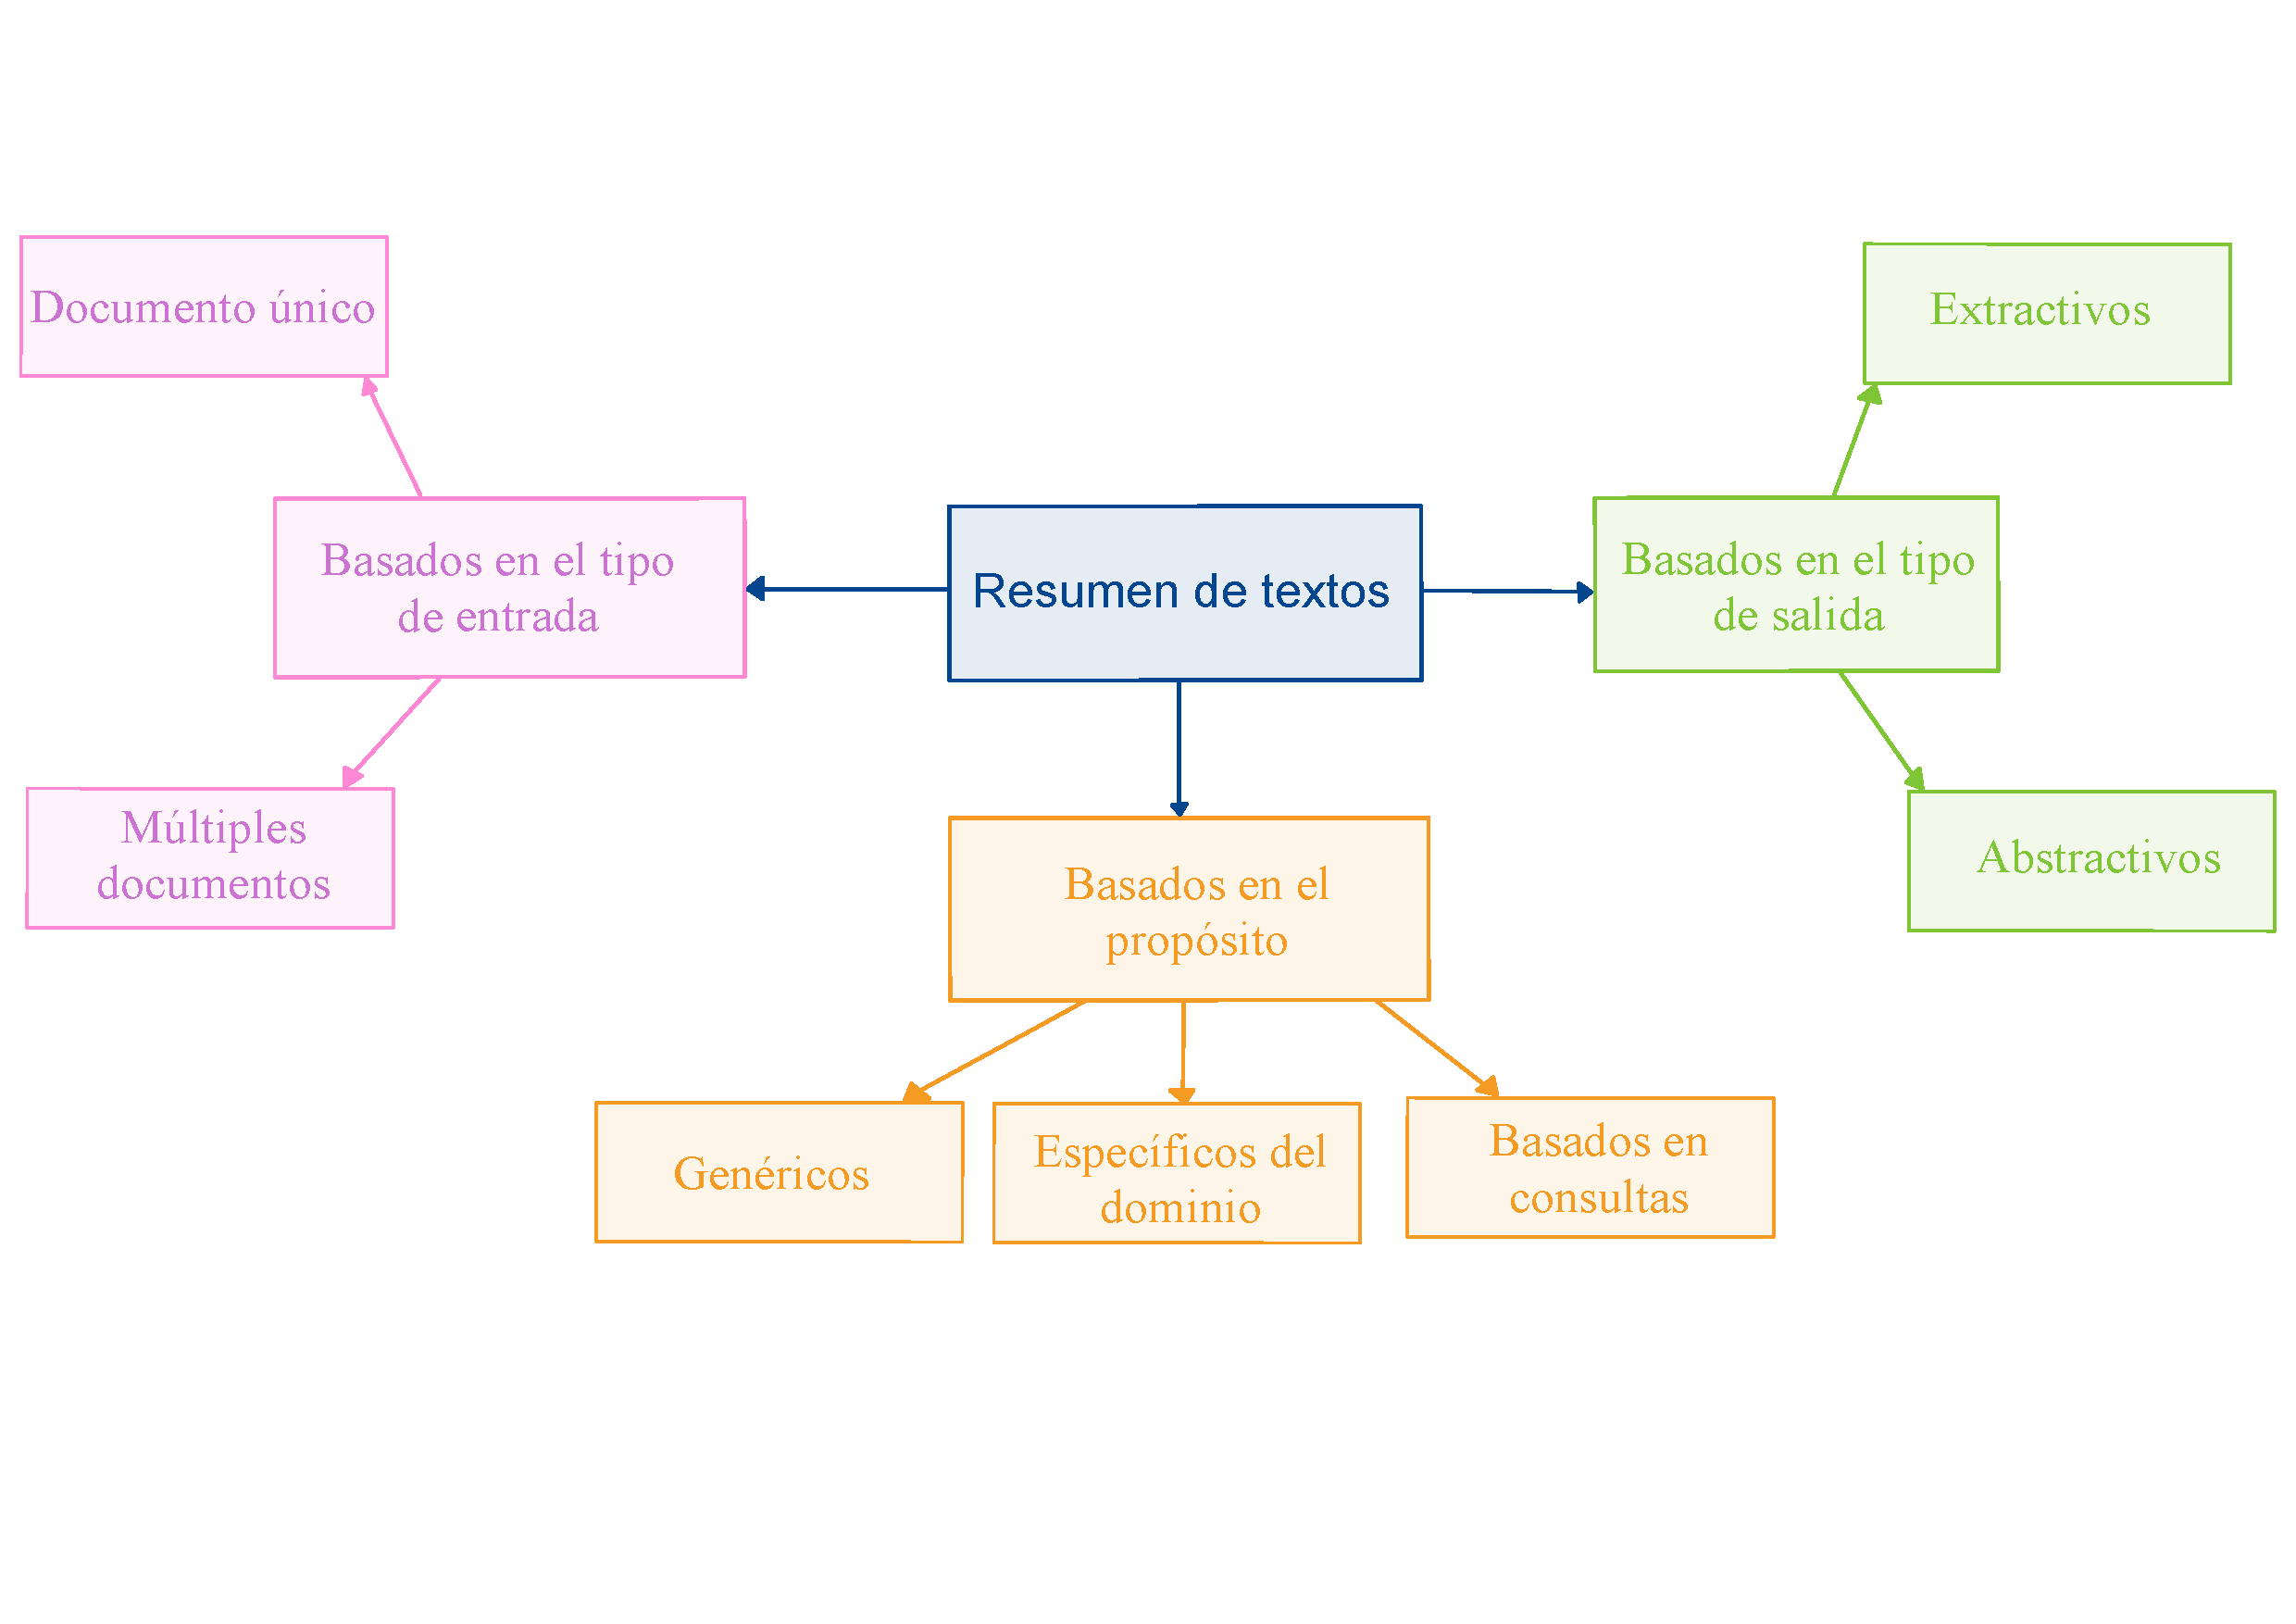
\includegraphics[width = 0.7\textwidth]{Imagenes/Vectorial/resumenTextos.pdf}
	\caption{Resumen de textos (adaptada de \cite{adhikari2020nlp})}
	\label{fig:resumenTextos}
\end{figure}

Los resúmenes extractivos son los que reutilizan las mismas frases existentes en el documento original, los abstractivos son más generales y se centran en los aspectos clave. De manera similar, las técnicas de resumen de un solo documento proporcionan resúmenes del texto de un solo documento, y las de múltiples documentos, generan resúmenes de varios documentos. Además, en la actualidad, hay una necesidad de resumir texto basándose en consultas. Los modelos de resumen basados en consultas proporcionan resúmenes del texto según un área específica descrita por la consulta proporcionada por el usuario, mientras que los resúmenes genéricos son en su mayoría resúmenes abstractos que se centran en el área general del texto de entrada.

\subsection{Impacto del desarrollo del PLN en la sociedad actual}

Como se ha visto, el procesamiento del lenguaje natural se ha desarrollado enormemente desde su concepción, especialmente en los últimos años. Con el uso de las tecnologías más modernas, se ha conseguido que el PLN sea parte del día a día de una persona común, lo cual ha traido múltiples beneficios a la sociedad, como pueden ser los siguientes:

\begin{itemize}
	\item \textbf{Mejora en la comunicación}: Facilitando la interacción con dispositivos electrónicos, como pueden ser los asistentes virtuales conocidos como Siri (de Apple) o Alexa (de Amazon). Además, al interpretar el lenguaje natural, se han creado diferentes dispositivos que permiten a personas con discapacidades, comunicarse con otra gente.
	
	\item \textbf{Progreso de la traducción automática}: Como se ha visto, la traducción automática tanto de discursos como de textos ha sido uno de los puntos de estudio principales relacionados con el PLN. A día de hoy, este ámbito está bastante desarrollado y permite unir personas de diferentes culturas y países.
	
	\item \textbf{Ayudas de soporte para negocios}: Con la proliferación de los conocidos 'chatbots', muchos negocios de todos los tamaños se han visto beneficiados, pudiendo incorporarlos como una medida de soporte para los clientes.
	
	\item \textbf{Análisis avanzado de datos}: El PLN permite utilizar enormes cantidades de texto y aportar estadísticas importantes a partir de él, lo cual sería muy difícil para os humanos debido a las grandes cantidades de información. Además, estos análisis a gran escala pueden servir para analizar los sentimientos de los mensajes publicados en redes sociales, por ejemplo.
	
\end{itemize}

A pesar de todas estas ventajas que el procesamiento del lenguaje natural ha aportado a la sociedad, existen varios desafíos para que esta tecnología sea capaz de funcionar. Las máquinas requieren una comunicación precisa y exacta, y los humanos hablamos con ambigüedades y de forma poco precisa en el día a día. Además, para poder transcribir a texto las palabras de una persona, es necesario un uso claro y comprensible del lenguaje. Estas solo son algunas de las barreras en las que se está trabajando para poder hacer esta tecnología accesible a todo el mundo.


\section{Interacción persona-ordenador}

(((Decir que está muy relacionada con el PLN)))
\subsection{Computación centrada en el humano}

\subsection{Extensibilidad y adaptación a todos los públicos}

\section{Relaciones sociales}

El artículo de \cite{park2023generative} sobre el que se ha basado la realización de este trabajo de fin de grado, está muy enfocado en el estudio del comportamiento humano y las finalidades que podría tener el hecho de simular relaciones sociales entre agentes de inteligenicia artificial. Algunos de los casos de uso de este estudio podrían ser la incorporación a personajes no jugables en videojuegos o la simulación de entornos reales para ver cómo afectaría la introducción de cambios en el ambiente, tal y como se menciona en el artículo.

Sin embargo, las relaciones sociales son un tema importante en la psicología y se han estudiado desde diferentes perspectivas. En la informática, el estudio de las relaciones sociales se ha centrado en la creación de sistemas que permitan la interacción social en línea. Es por eso que se divide el estudio de las relaciones sociales en estos dos campos, abordando en cada uno el contexto, la historia e investigaciones anteriores relacionadas con las relaciones sociales desde dos ámbitos diferentes.

\subsection{Psicología}

Las relaciones sociales desempeñan un papel fundamental en la vida humana, impactando de manera significativa en el bienestar emocional y mental de las personas. El estudio de las interacciones sociales ha revelado una serie de beneficios intrínsecos que estas conexiones ofrecen a nivel psicológico y emocional.

A lo largo del tiempo ha habido estudios que muestran de manera consistente que los individuos con menor cantidad de relaciones sociales son mas propensos a fallecer en comparación con lo que tienen una vida social plena. Estos estudios han arrojado una mayor evidencia en países industrializados \citep{House1988}.

Una vez se conoció el claro vínculo entre las relaciones sociales y la salud de las personas, los científicos se centraron en explicar cómo ocurre esto. Generalmente, existen tres amplias maneras en las que las relaciones sociales influencian la salud: de comportamiento, psicosociales y fisiológicas \citep{doi:10.1177/0022146510383501}.

\begin{itemize}
	\item \textbf{Explicaciones de comportamiento}: 
	Los comportamientos relacionados con la salud abarcan una amplia gama de conductas personales que influyen en la salud, la morbilidad y la mortalidad. De hecho, los comportamientos relacionados con la salud explican aproximadamente el 40 por ciento de la mortalidad prematura, así como una morbilidad y discapacidad sustanciales en los Estados Unidos. \citep{activePolicyAttention}
	
	\item \textbf{Explicaciones psicosociales}: La investigación en diferentes disciplinas y poblaciones sugiere la posibilidad de que algunos mecanismos psicosociales influyan en como los lazos sociales promueven la salud. Diferentes estudios han observado solamente uno de estos mecanismos, pero debido a la complejidad de la interconexión de estos mecanismos, hace que no sea posible llegar a una conclusión certera a no ser que se estudien todos a la vez.
	
	\item \textbf{Explicaciones fisiológicas}: Profesionales de varios ámbitos del mundo de la salud han  contribuido al entendimiento de algunas acciones (consumo excesivo de comida, de alcohol, de tabaco...) para reducir el estrés. Además, estas acciones muchas veces están relacionadas con actividades sociales y, el hecho de relacionarse con gente que exceda el consumo de estas sustancias, puede afectar gravemente a la salud.
	
	
\end{itemize}

Se ha visto que las relaciones sociales pueden ser muy positivas para la salud; sin embargo, también se ha comprobado que las relaciones sociales de mala calidad, también pueden afectar de manera negativa en la salud de las personas. Un matrinonio con problemas de comunicación o de entendimiento se ha asociado con funciones del sistema inmune o endocrino afectadas \citep{doi:10.1177/0265407500171001}.

\subsection{Informática a lo largo del tiempo}

((historia y estudios anteriores))

\subsubsection{Redes Sociales}
